
    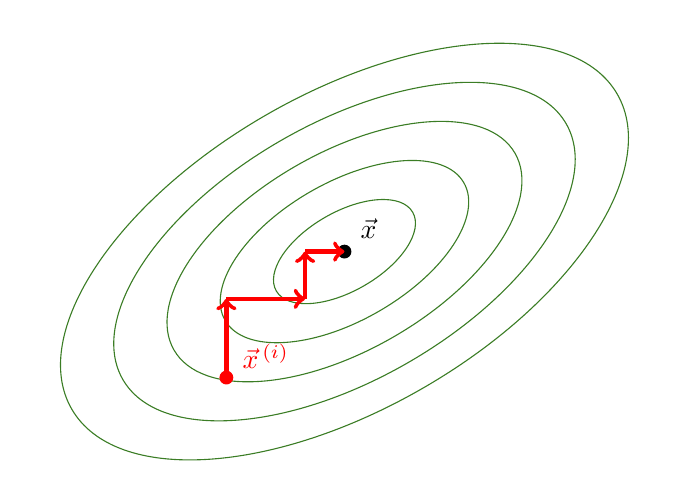
\begin{tikzpicture}
        \foreach \size in {1, 1.75, ..., 4} {
            \draw[OliveGreen, scale=\size, rotate=30] (0,0) ellipse (1cm and .5cm);
        };
        \node[circle, inner sep=0, minimum size=5pt,fill, label={30:$\vec{x}$}]() at (0,0){};

        \node[ red, circle, inner sep=0, minimum size=5pt, fill,
        label={[red, xshift=5mm, yshift=-1mm]$\vec{x}^{\,(i)}$}
        ] () at (-1.5, -1.6){};

        \draw[->, red, ultra thick] (-1.5, -1.6) -- (-1.5, -.6);
        \draw[->, red, ultra thick] (-1.5, -0.6) -- (-0.5, -0.6);
        \draw[->, red, ultra thick] (-0.5, -0.6) -- (-0.5, 0);
        \draw[->, red, ultra thick] (-0.5, 0) -- (0, 0);

    \end{tikzpicture}
